\documentclass[14pt]{memoir}

\usepackage{amsmath} %for equations in the document
\usepackage{graphicx} %for image inclusion
\usepackage{float} %for image placement
\usepackage{listings} %for code inclusion
\usepackage{color} %for code color
%\usepackage{fontspec}

%\setmainfont[Ligatures=TeX]{Segoe Print}
%\setmainfont[Ligatures=TeX]{Comic Sans}

\usepackage{kantlipsum}

\usepackage{duck}

\lstdefinestyle{customarduino}{belowcaptionskip = 1\baselineskip,
breaklines = true,
frame = L,
xleftmargin=\parindent,
language=C,
showstringspaces=false,
basicstyle=\footnotesize\ttfamily,
keywordstyle=\bfseries\color{green!40!black},
commentstyle=\itshape\color{purple!40!black},
identifierstyle=\color{blue},
stringstyle=\color{orange},
}

%\lstdefinestyle{customarduino}{
%belowcaptionskip=1\baselineskip,
%breaklines=true,
%frame=L,
%xleftmargin=\parindent,
%language=C,
%showstringspaces=false,
%basicstyle=\footnotesize\ttfamily,
%keywordstyle=\bfseries\color{green!40!black},
%commentstyle=\itshape\color{purple!40!black},
%identifierstyle=\color{blue},
%stringstyle=\color{orange},
%}


\begin{document}



\chapterstyle{weloveducks}

\setlength{\parskip}{1.5\baselineskip}
\setlength{\parindent}{0pt}
%\OnehalfSpacing{}
\chapter{The journey begins}
Hi, I am a duck. Quack! You'll see me a lot. I'll guide you
through the notes. Also, I hope you can see the flowers above,
they're there to show your progress. `Yaaaah!`

\section*{Introduction}
Voltage is the potential energy between two points in a circuit.
\\
Current is the rate of flow of charge in a circuit.
\\
Image a tank with water. Voltage is similar to the pressure in the
tank. The larger the tank, the more the pressure.
\\
Current is the rate of flow of the water when the tap is opened.
The larger the tank, the faster the water flows.
\\
Resistance is the tap. If is opened completely (similar to lower
resistance), the water will flow faster. If opened about halfway,
the water will flow slowly.
\\
The following equations will help you out a lot:
\begin{align}
    V &= I * R \\
    I &= \frac{V}{R}\\
    R &= \frac{V}{I}
\end{align}
\section*{LEDs}
LED is an electronic device that produces light when voltage and
current is supplied through it.
\\
It is stands for Light Emitting Diode.
\\
The following schematics show how to connect LEDs.
\begin{figure}[h]
    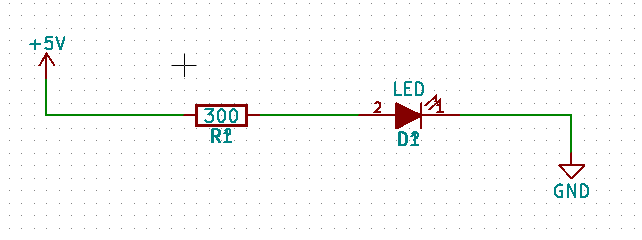
\includegraphics[width=\linewidth]{circuit_images/one_led.png}
    \caption{one led in a circuit}
\end{figure}
\begin{figure}[H]
    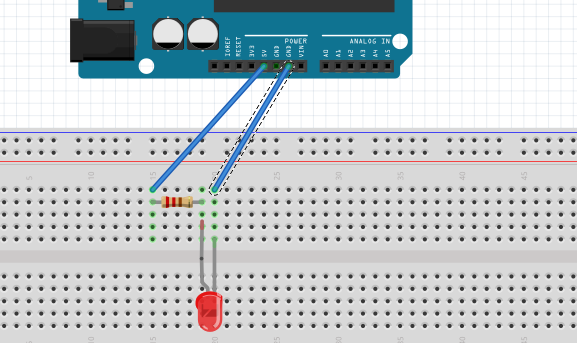
\includegraphics[width=0.7\linewidth]{./circuit_images/fritz_one_led.png}
    \caption{One LED in a circuit set up on breadboard}
\end{figure}

%TODO include fritzing cirtuitkk
\begin{figure}[H]
    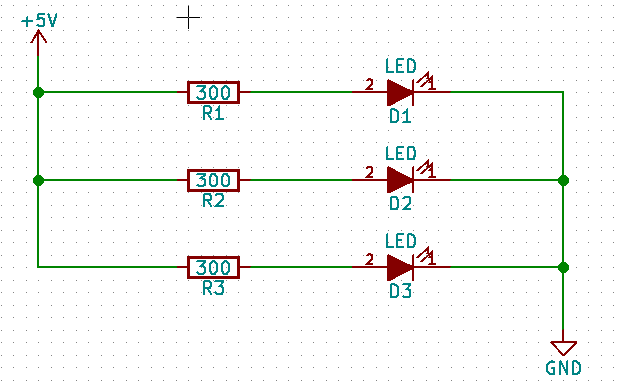
\includegraphics[width=0.7\linewidth]{circuit_images/multiple_leds.png}
    \caption{Multiple LEDs in a circuit}
\end{figure}

\section*{Programming LEDS}
Similar to the ciruits made in the previous section. However,
instead of directly supplying 5V to the LEDs, we will use the
arduinos Input Output pins to supply the power.
\\
For example make a circuit similar to the one led circuit. The
wire that comes from the 5V of the arduino, now place it in the
hole labelled 1 on the arduino.
\\
Then open the arduino software and write the following code:
\lstinputlisting[caption=BlinkingLED,
style=customarduino]{../codes/ledblink/ledblink.ino}

For multiple LEDs connect the circuit as shown below:
\begin{figure}[H]
    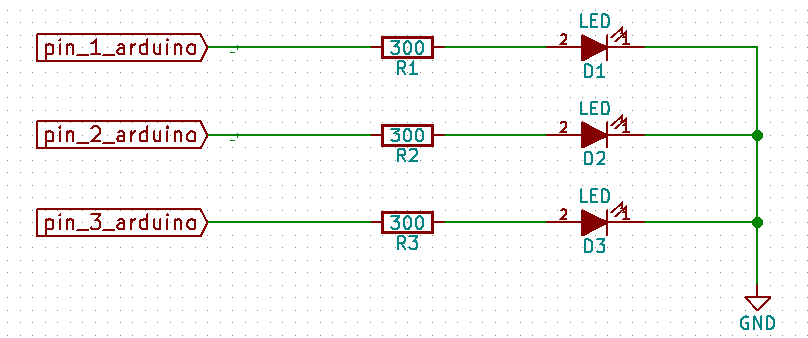
\includegraphics[width=\linewidth]{circuit_images/blinking_leds.png}
    \caption{Blinking LEDs in a circuit}
\end{figure}

Here is the code for the arduino:

\lstinputlisting[caption=Three Blinking LEDs,
style=customarduino]{../codes/threeleds/threeleds.ino}

And here is how the circuit should look like:
\begin{figure}[H]
    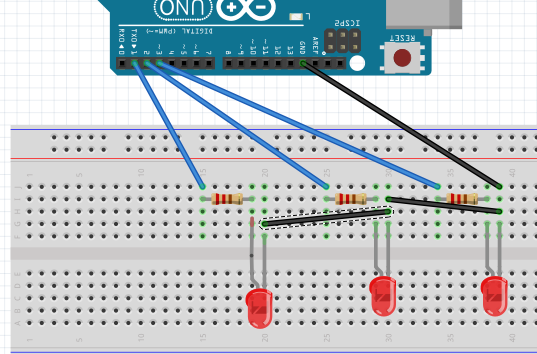
\includegraphics[width=0.7\linewidth]{circuit_images/fritz_blinking_leds.png}
    \caption{Blinking LEDs in a breadboard}
\end{figure}

\chapter{More about LEDs}
So we've made it to the next part. Yaah. This is a really
interesting section. We'll learn about sensors and use a buzzer.

\section*{RGB LED}
The RGB LED is different from the LEDs seen so far. It contains
four legs, three of the same size and one really long one.
\\
It also has three different colors: Reg, Green and Blue.
\\
If you connect the longest pin to ground and place resistors on
each of the other legs similar to the circuits made in the LED
section, that is assume each leg is the longest leg of a 2 pin
resistor, then provide 5V to each leg, you will see the different
colors.
\\
\begin{figure}[H]
    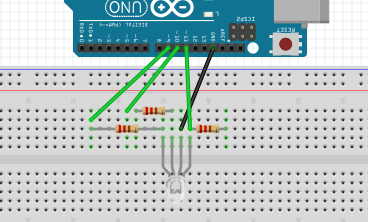
\includegraphics[width=\linewidth]{circuit_images/rgb_led.png}
    \caption{RGB LED in a circuit}
\end{figure}

The following is the code used:
\lstinputlisting[caption=BlinkingLED,
style=customarduino]{../codes/rgbled/rgbled.ino}


\section*{Infra Red LEDs}
%TODO chris to provide info

\section*{Buzzer}
The buzzer is almost like a small speaker.
\\
When a changing voltage is applied to it, it will produce sound or
a tone.
\\
The arduino software has an example that runs of the buzzer.
\\
To access this, go to `File' -> `Examples' -> `Digital' ->
`toneMelody'
\\
Here is the circuit that works with the given example:
\begin{figure}[h]
    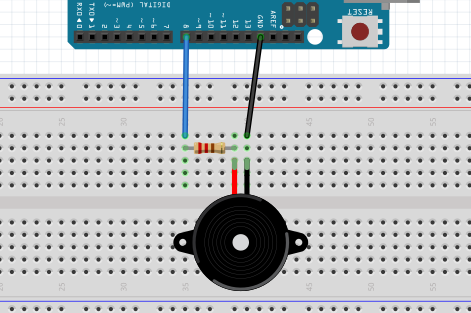
\includegraphics[width=\linewidth]{circuit_images/buzzer.png}
    \caption{Buzzer circuit}
\end{figure}

\chapter{Now what}
It's feels as though we've learned so much in so little time. What
else can we learn?

\section*{Servo Motor}
A servo motor is a motor that can be precisely controlled.\\
%include image
\begin{figure}[h]
    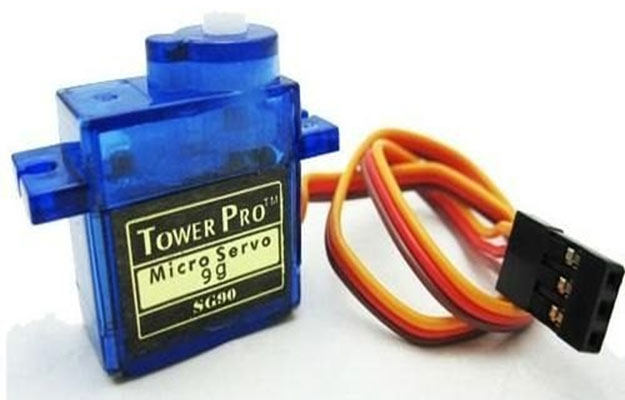
\includegraphics[width=\linewidth]{./circuit_images/servo_motor.jpg}
    \caption{Buzzer circuit}
\end{figure}

To connect the servo, it should have three differenly coloured
wired:
\begin{enumerate}
    \item Red: this goes to 5V
    \item Orange: this goes to a PWM pin, that is a pin with `~'
        sign on it.
    \item Brown or Black: this goes to GND
\end{enumerate}

The arduino software has an example that runs of the servo.
\\
To access this, go to `File' -> `Examples' -> `Servo' ->
`sweep'
\section*{DC Motor}



\chapter{More about motors}


\end{document}
